\documentclass[11pt]{article}
\usepackage{geometry,marginnote} % Pour passer au format A4
\geometry{hmargin=1cm, vmargin=1cm} % 

% Page et encodage
\usepackage[T1]{fontenc} % Use 8-bit encoding that has 256 glyphs
\usepackage[english,french]{babel} % Français et anglais
\usepackage[utf8]{inputenc} 

\usepackage{lmodern,numprint}
\setlength\parindent{0pt}

% Graphiques
\usepackage{graphicx,float,grffile,units}
\usepackage{tikz,pst-eucl,pst-plot,pstricks,pst-node,pstricks-add,pst-fun,pgfplots} 

% Maths et divers
\usepackage{amsmath,amsfonts,amssymb,amsthm,verbatim}
\usepackage{multicol,enumitem,url,eurosym,gensymb,tabularx}

\DeclareUnicodeCharacter{20AC}{\euro}



% Sections
\usepackage{sectsty} % Allows customizing section commands
\allsectionsfont{\centering \normalfont\scshape}

% Tête et pied de page
\usepackage{fancyhdr} \pagestyle{fancyplain} \fancyhead{} \fancyfoot{}

\renewcommand{\headrulewidth}{0pt} % Remove header underlines
\renewcommand{\footrulewidth}{0pt} % Remove footer underlines

\newcommand{\horrule}[1]{\rule{\linewidth}{#1}} % Create horizontal rule command with 1 argument of height

\newcommand{\Pointilles}[1][3]{%
  \multido{}{#1}{\makebox[\linewidth]{\dotfill}\\[\parskip]
}}

\newtheorem{Definition}{Définition}

\usepackage{siunitx}
\sisetup{
    detect-all,
    output-decimal-marker={,},
    group-minimum-digits = 3,
    group-separator={~},
    number-unit-separator={~},
    inter-unit-product={~}
}

\setlength{\columnseprule}{1pt}

\begin{document}

\textbf{Nom, Prénom :} \hspace{8cm} \textbf{Classe :} \hspace{3cm} \textbf{Date :}\\

\vspace{-0.5cm} \begin{center}
  \textit{La valeur morale ne peut pas être remplacée par la valeur intelligence et j'ajouterai : Dieu merci !}  - \textbf{Albert Einstein}
\end{center}

\subsection*{Nv 1 - Connaissances}

\begin{itemize}[label={$\bullet$}]
  \item Aire d'un carré de côté c : \dotfill
  \item Aire d'un rectangle de longueur l et de largeur L : \dotfill
  \item Aire d'un triangle de base b et de hauteur h : \dotfill
  \item Aire d'un cercle de rayon R :\dotfill
\end{itemize} 

\textbf{Calculer les aires grises. Écrire les calculs. Mettre l'unité dans la réponse.}

\subsection*{Nv 2 - Aires simples}

\begin{multicols}{3}
  
\begin{figure}[H]
  \centering
  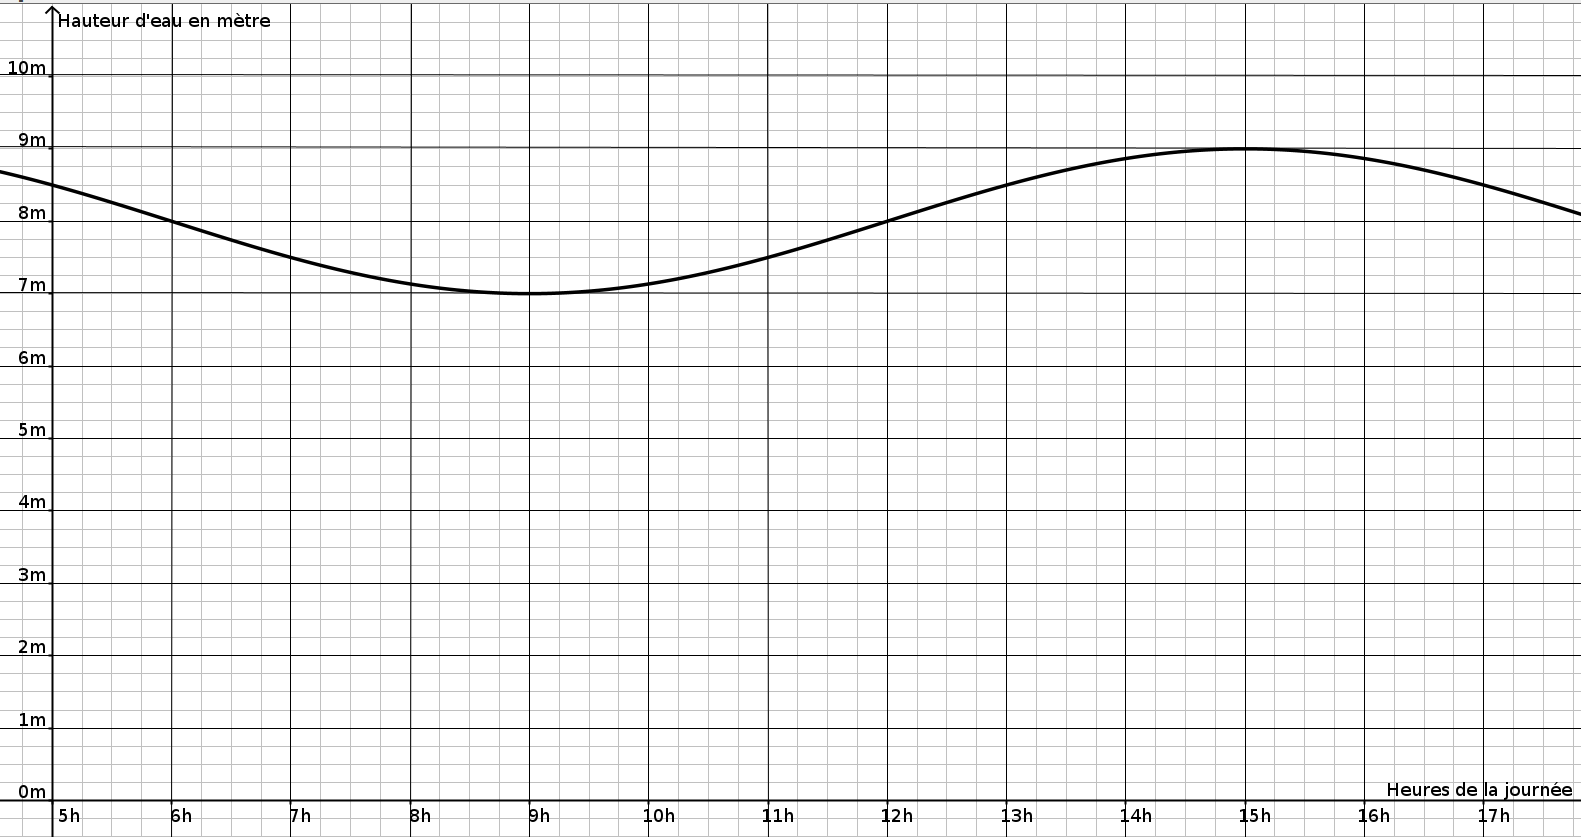
\includegraphics[width=\linewidth]{5x8-aires/ex1.pdf}
\end{figure}

\begin{figure}[H]
  \centering
  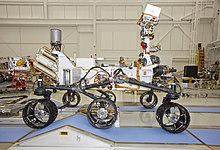
\includegraphics[width=0.8\linewidth]{5x8-aires/ex3.pdf}
\end{figure}

\begin{figure}[H]
  \centering
  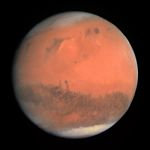
\includegraphics[width=0.8\linewidth]{5x8-aires/ex4.pdf}
\end{figure}

\end{multicols}

\Pointilles[20]

\newpage

\subsection*{Nv 3 - Aires composées}

\begin{multicols}{3}

\begin{figure}[H]
  \centering
  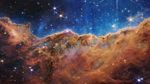
\includegraphics[width=0.7\linewidth]{5x8-aires/ex6.pdf}
\end{figure}

\begin{figure}[H]
  \centering
  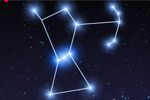
\includegraphics[width=0.7\linewidth]{5x8-aires/ex7.pdf}
\end{figure}

\begin{figure}[H]
  \centering
  \includegraphics[width=0.7\linewidth]{5x8-aires/ex8.pdf}
\end{figure}

\end{multicols}

\Pointilles[20]

\subsection*{Nv 4 - Aires complexes}

\textbf{Calculer l'aire du carré. Calculer l'aire des 4 demi-cercles. En déduire l'aire les pétales gris.}

\begin{minipage}[t]{0.25\textwidth}
\begin{figure}[H]
  \centering
  \includegraphics[width=0.8\linewidth]{5x8-aires/ex9.pdf}
\end{figure}
\end{minipage}
\begin{minipage}[t]{0.75\textwidth}
  \Pointilles[10]
\end{minipage}
\end{document}
